\item \points{25} {\bf Linear Classifiers (logistic regression and GDA)}

In this problem, we cover two probabilistic linear classifiers we have covered in class so far. First, a discriminative linear classifier: logistic regression. Second, a generative linear classifier: Gaussian discriminant analysis (GDA). Both the algorithms find a linear decision boundary that separates the data into two classes, but make different assumptions. Our goal in this problem is to get a deeper understanding of the similarities and differences (and, strengths and weaknesses) of these two algorithms.

For this problem, we will consider two datasets, along with starter codes provided in the following files:
\begin{center}
\begin{itemize} %[label=\roman*.]
	\item \texttt{linearclass/src/ds1\_{train,valid}.csv}
	\item \texttt{linearclass/src/ds2\_{train,valid}.csv}
        \item \texttt{linearclass/src/logreg.py}
        \item \texttt{linearclass/src/gda.py}
\end{itemize}
\end{center}
Each file contains $\nexp$ examples, one example $(x^{(i)}, y^{(i)})$ per row. In particular, the $i$-th row contains columns $x^{(i)}_0\in\Re$, $x^{(i)}_1\in\Re$, and $y^{(i)}\in\{0, 1\}$. In the subproblems that follow, we will investigate using logistic regression and Gaussian discriminant analysis (GDA) to perform binary classification on these two datasets.

\begin{enumerate}
	\item \subquestionpointswritten{6}

In lecture we saw the average empirical loss for logistic regression:
\begin{equation*}
	J(\theta)
	= -\frac{1}{\nexp} \sum_{i=1}^\nexp \left(y^{(i)}\log(h_{\theta}(x^{(i)}))
		+  (1 - y^{(i)})\log(1 - h_{\theta}(x^{(i)}))\right),
\end{equation*}
where $y^{(i)} \in \{0, 1\}$, $h_\theta(x) = g(\theta^T x)$ and $g(z) = 1 / (1 + e^{-z})$.

Find the Hessian $H$ of this function, and show that for any vector $z$, it holds true that
%
\begin{equation*}
    z^T H z \ge 0.
\end{equation*}
%
{\bf Hint:} You may want to start by showing that $\sum_i\sum_j z_i x_i x_j z_j = (x^Tz)^2 \geq 0$. Recall also that $g'(z) = g(z)(1-g(z))$.

{\bf Remark:} This is one of the standard ways of showing that the matrix $H$ is positive semi-definite, written ``$H \succeq 0$.''  This implies that $J$ is convex, and has no local minima other than the global one. If you have some other way of showing $H \succeq 0$, you're also welcome to use your method instead of the one above.\clearpage

{\bf BEGIN PROOF HERE}\\

Since $g'(z) = g(z)(1-g(z))$ and $h(x) = g(\theta^T x)$, it follows that $\partial h(x) / \partial \theta_k = h(x)(1 - h(x)) x_k$.

Letting $h_{\theta}(x^{(i)}) = g(\theta^T x^{(i)})
= 1/(1 + \exp(-\theta^T x^{(i)})$, we have\\

\begin{flalign*}
	\frac{\partial\log h_{\theta}(x^{(i)})}{\partial\theta_k} \\
	&= \frac{\partial\log g(\theta^T x^{(i)})}{\partial\theta_k} \\
	&= \frac{1}{g(\theta^T x^{(i)})}\frac{\partial g(\theta^T x^{(i)})}{\partial\theta_k} \\
	&= \frac{1}{g(\theta^T x^{(i)})}g(\theta^T x^{(i)})(1-g(\theta^T x^{(i)})) \frac{\partial (\theta^T x^{(i)})}{\partial\theta_k} \\
	 &= (1-g(\theta^T x^{(i)}))x_k^{(i)}
	  & & & & &\\[50pt]
	\frac{\partial\log(1 - h_{\theta}(x^{(i)}))}{\partial\theta_k} \\
	&= \frac{\partial\log(1 - g(\theta^T x^{(i)}))}{\partial\theta_k} \\
	&= \frac{-1}{1 - g(\theta^T x^{(i)})}\frac{\partial g(\theta^T x^{(i)})}{\partial\theta_k} \\
	&= \frac{-1}{1 - g(\theta^T x^{(i)})}g(\theta^T x^{(i)})(1-g(\theta^T x^{(i)}))\frac{\partial (\theta^T x^{(i)})}{\partial\theta_k} \\
	&= -g(\theta^T x^{(i)})x_k^{(i)}
	 & & & &
	\\[50pt]
\end{flalign*}

Substituting into our equation for $J(\theta)$, we have
%
\begin{flalign*}
	\frac{\partial J(\theta)}{\partial\theta_k} \\
	&= \frac{\partial}{\partial\theta_k}\frac{-1}{\nexp} \sum_{i=1}^\nexp \left(y^{(i)}\log(h_{\theta}(x^{(i)}))
		+  (1 - y^{(i)})\log(1 - h_{\theta}(x^{(i)}))\right) \\
	&=  \frac{-1}{\nexp} \sum_{i=1}^\nexp \left(y^{(i)}\frac{\partial}{\partial\theta_k}\log(h_{\theta}(x^{(i)}))
		+  (1 - y^{(i)})\frac{\partial}{\partial\theta_k}\log(1 - h_{\theta}(x^{(i)}))\right) \\
	&= \frac{-1}{\nexp} \sum_{i=1}^\nexp \left(y^{(i)} (1-g(\theta^T x^{(i)}))x_k^{(i)}
		+  (1 - y^{(i)})(-g(\theta^T x^{(i)})x_k^{(i)})\right) \\\\
	&= \frac{-1}{\nexp} \sum_{i=1}^\nexp \left(y^{(i)}x_k^{(i)} 
		- y^{(i)}g(\theta^T x^{(i)})x_k^{(i)} + y^{(i)}g(\theta^T x^{(i)})x_k^{(i)}
		- g(\theta^T x^{(i)})x_k^{(i)} \right) \\
	&= \frac{-1}{\nexp} \sum_{i=1}^\nexp \left(y^{(i)}x_k^{(i)} -g(\theta^T x^{(i)})x_k^{(i)} \right) \\
	&= \frac{-1}{\nexp} \sum_{i=1}^\nexp \left(y^{(i)}-g(\theta^T x^{(i)}) \right)x_k^{(i)}
	 & & &\\[50pt]
\end{flalign*}
%

Consequently, the $(k, l)$ entry of the Hessian is given by
%
\begin{flalign*}
	H_{kl} \\
	&= \frac{\partial^2 J(\theta)}{\partial\theta_k\partial\theta_l} \\
	&= \frac{\partial}{\partial\theta_l}\frac{\partial J(\theta)}{\partial\theta_k}\\
	&= \frac{\partial}{\partial\theta_l}
		\frac{-1}{\nexp} \sum_{i=1}^\nexp \left(y^{(i)}-g(\theta^T x^{(i)}) \right)x_k^{(i)} \\
	&= \frac{1}{\nexp} \sum_{i=1}^\nexp \frac{\partial}{\partial\theta_l} g(\theta^T x^{(i)})x_k^{(i)} \\
	&= \frac{1}{\nexp} \sum_{i=1}^\nexp g(\theta^T x^{(i)})(1-g(\theta^T x^{(i)}))x_k^{(i)} \frac{\partial}{\partial\theta_l}(\theta^T x^{(i)}) \\
	&= \frac{1}{\nexp} \sum_{i=1}^\nexp g(\theta^T x^{(i)})(1-g(\theta^T x^{(i)}))x_k^{(i)}x_l^{(i)}\\
	 & & & & &\\[50pt]
\end{flalign*}
%

Using the fact that $X_{ij} = x_i x_j$ if and only if $X = xx^T$, we have
%
\begin{flalign*}
	H \\
	&= \sum_k\sum_l H_{kl} \\
	&= \sum_k\sum_l \frac{1}{\nexp} \sum_{i=1}^\nexp g(\theta^T x^{(i)})(1-g(\theta^T x^{(i)}))x_k^{(i)}x_l^{(i)}
	 & & & & & & &\\[50pt]
\end{flalign*}

To prove that $H$ is positive semi-definite, show $z^T Hz \ge 0$ for all $z\in\Re^\di$.
%
\begin{flalign*}
	z^T H z \\
	& = \sum_k\sum_l \frac{1}{\nexp} \sum_{i=1}^\nexp g(\theta^T x^{(i)})(1-g(\theta^T x^{(i)}))z_k x_k^{(i)}x_l^{(i)} z_l \\
	&=  \frac{1}{\nexp} \sum_{i=1}^\nexp g(\theta^T x^{(i)})(1-g(\theta^T x^{(i)})) \sum_k\sum_l z_k x_k^{(i)}x_l^{(i)} z_l \\
	&= \frac{1}{\nexp} \sum_{i=1}^\nexp g(\theta^T x^{(i)})(1-g(\theta^T x^{(i)})) (x^T z)^2 
	& & & & & &\\[50pt]
\end{flalign*}
%
$g(\theta^T x^{(i)})$ is sigmoid with value between 0 and 1; and $(x^T z)^2 \geq 0$; therefore, $H \succeq 0$. \\\\

{\bf END PROOF}\\
        \ifnum\solutions=1 {
            \input{linearclass/01-logreg-sol}
        } \fi

	\item \subquestionpointscoding{2}
Follow the instructions in \texttt{linearclass/src/logreg.py} to train a logistic regression classifier using Newton's Method. Starting with $\theta = \vec{0}$, run Newton's Method until the updates to $\theta$ are small: Specifically,  train until the first iteration $k$ such that $\|\theta_{k} - \theta_{k-1}\|_1 < \epsilon$, where $\epsilon = 1\times 10^{-5}$. Make sure to write your model's predicted probabilities on the validation set to the file specified in the code.

To verify a correct implementation, consider creating a plot of the \textbf{validation data} with $x_1$ on the horizontal axis and $x_2$ on the vertical axis. To visualize the two classes, use a different symbol for examples $x^{(i)}$ with $y^{(i)} = 0$ than for those with $y^{(i)} = 1$. On the same figure, plot the decision boundary found by logistic regression (i.e, line corresponding to $p(y|x) = 0.5$).

Your plot should look similar to the following:

\begin{figure}[H]
	\centering
	\vspace{2mm}
	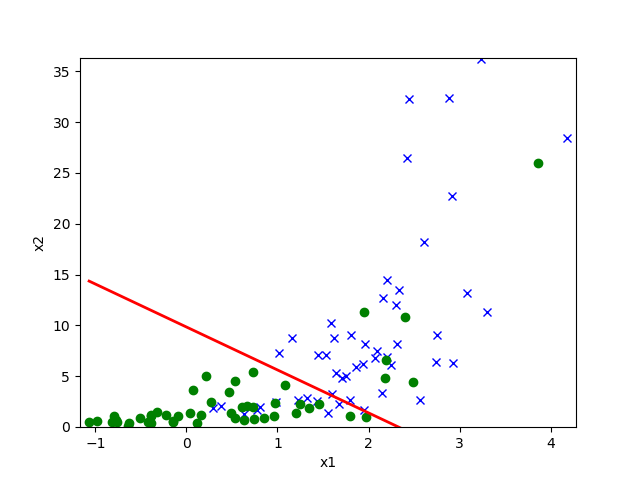
\includegraphics[width=0.65\linewidth]{linearclass/src/p01b_pred_1.png}
    \caption{Separating hyperplane for logistic regression on Dataset 1}
\end{figure}

        \ifnum\solutions=1 {
            \input{linearclass/02-solve-logreg-sol}
        } \fi


	\item \subquestionpointswritten{4}
Recall that in GDA we model the joint distribution of $(x, y)$ by the following
equations:
%
\begin{eqnarray*}
	p(y) &=& \begin{cases}
	\phi & \mbox{if~} y = 1 \\
	1 - \phi & \mbox{if~} y = 0 \end{cases} \\
	p(x | y=0) &=& \frac{1}{(2\pi)^{\di/2} |\Sigma|^{1/2}}
		\exp\left(-\frac{1}{2}(x-\mu_{0})^T \Sigma^{-1} (x-\mu_{0})\right) \\
	p(x | y=1) &=& \frac{1}{(2\pi)^{\di/2} |\Sigma|^{1/2}}
		\exp\left(-\frac{1}{2}(x-\mu_1)^T \Sigma^{-1} (x-\mu_1) \right),
\end{eqnarray*}
%
where $\phi$, $\mu_0$, $\mu_1$, and $\Sigma$ are the parameters of our model.

Suppose we have already fit $\phi$, $\mu_0$, $\mu_1$, and $\Sigma$, and now
want to predict $y$ given a new point $x$. To show that GDA results in a
classifier that has a linear decision boundary, show the posterior distribution
can be written as
%
\begin{equation*}
	p(y = 1\mid x; \phi, \mu_0, \mu_1, \Sigma)
	= \frac{1}{1 + \exp(-(\theta^T x + \theta_0))},
\end{equation*}
%
where $\theta\in\Re^\di$ and $\theta_{0}\in\Re$ are appropriate functions of
$\phi$, $\Sigma$, $\mu_0$, and $\mu_1$.\\

{\bf BEGIN PROOF HERE}\\

For shorthand, we let $\mc{H} = \{\phi, \Sigma, \mu_{0}, \mu_1\}$ denote
the parameters for the problem.
Since the given formulae are conditioned on $y$, use Bayes rule to get:
\begin{align*}
	p(y =1| x ; & \mc{H})\\
	& = \frac {p(x|y=1; \mc{H}) p(y=1; \mc{H})} {p(x; \mc{H})}\\
	& = \frac {p(x|y=1; \mc{H}) p(y=1; \mc{H})}
		{p(x|y=1; \mc{H}) p(y=1; \mc{H}) + p(x|y={0}; \mc{H}) p(y={0};
		\mc{H})}\\\\
	&= \frac{\frac{1}{(2\pi)^{\di/2} |\Sigma|^{1/2}}
		\exp\left(-\frac{1}{2}(x-\mu_1)^T \Sigma^{-1} (x-\mu_1) \right) \phi} 
		{
		\frac{1}{(2\pi)^{\di/2} |\Sigma|^{1/2}}
		\exp\left(-\frac{1}{2}(x-\mu_1)^T \Sigma^{-1} (x-\mu_1) \right) \phi
		+ \frac{1}{(2\pi)^{\di/2} |\Sigma|^{1/2}}
		\exp\left(-\frac{1}{2}(x-\mu_{0})^T \Sigma^{-1} (x-\mu_{0})\right) (1-\phi)
		} \\
	&=  \frac{
		\exp\left(-\frac{1}{2}(x-\mu_1)^T \Sigma^{-1} (x-\mu_1) \right) \phi} 
		{
		\exp\left(-\frac{1}{2}(x-\mu_1)^T \Sigma^{-1} (x-\mu_1) \right) \phi
		+ 
		\exp\left(-\frac{1}{2}(x-\mu_{0})^T \Sigma^{-1} (x-\mu_{0})\right) (1-\phi)
		} \\
	&= \frac{
		1} 
		{
		1
		+ 
		\frac{\exp\left(-\frac{1}{2}(x-\mu_{0})^T \Sigma^{-1} (x-\mu_{0})\right) (1-\phi)}{\exp\left(-\frac{1}{2}(x-\mu_1)^T \Sigma^{-1} (x-\mu_1) \right) \phi}
		}\\
	&= \frac{1} {1+ 
		\frac{\exp\left(-\frac{1}{2}(x-\mu_{0})^T \Sigma^{-1} (x-\mu_{0})\right) \exp(\log(1-\phi))}{\exp\left(-\frac{1}{2}(x-\mu_1)^T \Sigma^{-1} (x-\mu_1) \right) \exp(\log(\phi))}
		}\\
	&= \frac{1} {1+ 
		\exp\left(-\frac{1}{2}(x-\mu_{0})^T \Sigma^{-1} (x-\mu_{0})
		+ \frac{1}{2}(x-\mu_1)^T \Sigma^{-1} (x-\mu_1) +\log((1-\phi)/\phi)
		\right) 
		}\\
	&= \frac{1} {1+ 
		\exp\left(-\frac{1}{2}(x^T-\mu_{0}^T) \Sigma^{-1} (x-\mu_{0})
		+ \frac{1}{2}(x^T-\mu_1^T) \Sigma^{-1} (x-\mu_1) +\log((1-\phi)/\phi)
		\right) 
		}\\
	&= \frac{1} {1+ 
		\exp\left(D +\log((1-\phi)/\phi)
		\right) 
		}\\
\end{align*}


\begin{align*}
D &= -\frac{1}{2}(x^T-\mu_{0}^T) \Sigma^{-1} (x-\mu_{0})
		+ \frac{1}{2}(x^T-\mu_1^T) \Sigma^{-1} (x-\mu_1) \\
	&= -\frac{1}{2}(x^T\Sigma^{-1}x -x^T\Sigma^{-1}\mu_{0}
			-\mu_{0}^T\Sigma^{-1}x + \mu_{0}^T\Sigma^{-1}\mu_{0})
			+ \frac{1}{2}(x^T\Sigma^{-1}x -x^T\Sigma^{-1}\mu_{1}
			-\mu_{1}^T\Sigma^{-1}x + \mu_{1}^T\Sigma^{-1}\mu_{1})
			\\
	&= -\frac{1}{2}(x^T\Sigma^{-1}\mu_{1} - x^T\Sigma^{-1}\mu_{0}
		+\mu_{1}^T\Sigma^{-1}x - \mu_{0}^T\Sigma^{-1}x
		+ \mu_{0}^T\Sigma^{-1}\mu_{0} - \mu_{1}^T\Sigma^{-1}\mu_{1})\\
	&= -\frac{1}{2}(x^T\Sigma^{-1}(\mu_{1}-\mu_{0})
		+ (\mu_{1}-\mu_{0})^T\Sigma^{-1}x
		+ \mu_{0}^T\Sigma^{-1}\mu_{0} - \mu_{1}^T\Sigma^{-1}\mu_{1}
		) \\
	&= -\frac{1}{2}(2(\mu_{1}-\mu_{0})^T\Sigma^{-1}x
		+ \mu_{0}^T\Sigma^{-1}\mu_{0} - \mu_{1}^T\Sigma^{-1}\mu_{1}
		) \\ 
	&= -(\mu_{1}-\mu_{0})^T\Sigma^{-1}x
		+ \frac{1}{2}(\mu_{1}^T\Sigma^{-1}\mu_{1} - \mu_{0}^T\Sigma^{-1}\mu_{0}
		)\\
	 &\\[100pt]
\end{align*}

\begin{align*}
p(y =1| x ; & \mc{H})\\
	&= \frac{1} {1+ 
		\exp\left(-(\mu_{1}-\mu_{0})^T\Sigma^{-1}x
		+ \frac{1}{2}(\mu_{1}^T\Sigma^{-1}\mu_{1} - \mu_{0}^T\Sigma^{-1}\mu_{0}) +\log((1-\phi)/\phi)
		\right) 
		}\\
	&= \frac{1} {1+ 
		\exp\left(-\left(\mu_{1}-\mu_{0})^T\Sigma^{-1}x
		+ \frac{1}{2}(\mu_{0}^T\Sigma^{-1}\mu_{0} - \mu_{1}^T\Sigma^{-1}\mu_{1}) -\log((1-\phi)/\phi)\right)
		\right) 
		}
	&
	 &\\[100pt]
\end{align*}

\begin{align*}
\theta^T &= (\mu_{1}-\mu_{0})^T\Sigma^{-1} \\
\theta_0 &= \frac{1}{2}(\mu_{0}^T\Sigma^{-1}\mu_{0} - \mu_{1}^T\Sigma^{-1}\mu_{1}) -\log((1-\phi)/\phi) 
	&
	 &\\[100pt]
\end{align*}

{\bf END PROOF}\\
        \ifnum\solutions=1 {
            \input{linearclass/03-gda-sol}
        }\fi

	\item \subquestionpointswritten{5} Given the dataset, we claim that the maximum likelihood estimates of the parameters are given by
\begin{eqnarray*}
    \phi &=& \frac{1}{\nexp} \sum_{i=1}^\nexp 1\{y^{(i)} = 1\} \\
    \mu_{0} &=& \frac{\sum_{i=1}^\nexp 1\{y^{(i)} = {0}\} x^{(i)}}{\sum_{i=1}^\nexp 1\{y^{(i)} = {0}\}} \\
    \mu_1 &=& \frac{\sum_{i=1}^\nexp 1\{y^{(i)} = 1\} x^{(i)}}{\sum_{i=1}^\nexp 1\{y^{(i)} = 1\}} \\
    \Sigma &=& \frac{1}{\nexp} \sum_{i=1}^\nexp (x^{(i)} - \mu_{y^{(i)}}) (x^{(i)} - \mu_{y^{(i)}})^T
\end{eqnarray*}
The log-likelihood of the data is
\begin{eqnarray*}
    \ell(\phi, \mu_{0}, \mu_1, \Sigma) &=& \log \prod_{i=1}^\nexp p(x^{(i)} , y^{(i)}; \phi, \mu_{0}, \mu_1, \Sigma) \\
    &=& \log \prod_{i=1}^\nexp p(x^{(i)} | y^{(i)}; \mu_{0}, \mu_1, \Sigma) p(y^{(i)}; \phi).
\end{eqnarray*}
By maximizing $\ell$ with respect to the four parameters, prove that the maximum likelihood estimates of $\phi$, $\mu_{0}, \mu_1$, and $\Sigma$ are indeed as given in the formulas above.  (You may assume that there is at least one positive and one negative example, so that the denominators in the definitions of $\mu_{0}$ and $\mu_1$ above are non-zero.)\\\\

{\bf BEGIN PROOF HERE}\\

First, derive the expression for the log-likelihood of the training data:
\begin{flalign*}
  \ell(\phi, \mu_{0}, \mu_1, \Sigma) \\
  &= \log \prod_{i=1}^\nexp p(x^{(i)} | y^{(i)}; \mu_{0}, \mu_1, \Sigma) p(y^{(i)}; \phi)\\
  &= \sum_{i=1}^{\nexp} \log p(x^{(i)} | y^{(i)}; \mu_{0}, \mu_1, \Sigma) +
  \sum_{i=1}^{n} \log p(y^{(i)}; \phi)\\\\
  &= \sum_{i=1}^{\nexp} \log \left( \frac{1}{(2\pi)^{n/2} |\Sigma|^{1/2}}
    \exp\left(-\frac{1}{2}(x^{(i)}-\mu_{y^{(i)}})^T \Sigma^{-1} (x^{(i)}-\mu_{y^{(i)}})\right)
    \right)
    + \sum_{i=1}^{\nexp} \log \left( \phi^{y^{(i)}}(1-\phi)^{(1-{y^{(i)}})}
    \right) \\
  &= \sum_{i=1}^{\nexp} -\frac{n}{2} \log(2\pi) - \frac{1}{2}\log(|\Sigma|)
    -\frac{1}{2}(x^{(i)}-\mu_{y^{(i)}})^T \Sigma^{-1} (x^{(i)}-\mu_{y^{(i)}})
    + y^{(i)}\log(\phi) +(1-y^{(i)})\log(1-\phi)
   & & & & & & &\\[50pt]
\end{flalign*}

Now, the likelihood is maximized by setting the derivative (or gradient) with respect to each of the parameters to zero.\\

\textbf{For $\mathbf{\phi}$:}

\begin{flalign*}
  \frac{\partial \ell}{\partial \phi} \\
  &= \frac{\partial}{\partial \phi} \sum_{i=1}^{\nexp} y^{(i)}\log(\phi) +(1-y^{(i)})\log(1-\phi) \\
  &= \sum_{i=1}^{\nexp} \frac{y^{(i)}}{\phi} - \frac{(1-y^{(i)})}{(1-\phi)} \\\\
& &\\[50pt]
\end{flalign*}

Setting this equal to zero and solving for $\phi$ gives the maximum
likelihood estimate.\\
\begin{flalign*}
  0 &= \sum_{i=1}^{\nexp} \frac{1\{y^{(i)} = 1\}}{\phi} - \frac{(1-1\{y^{(i)} = 1\})}{(1-\phi)} \\
  &= \frac{\sum_{i=1}^{\nexp} 1\{y^{(i)} = 1\}}{\phi} - \frac{(n- \sum_{i=1}^{\nexp}1\{y^{(i)} = 1\})}{(1-\phi)} \\
  &= \sum_{i=1}^{\nexp} 1\{y^{(i)} = 1\} - \phi\sum_{i=1}^{\nexp} 1\{y^{(i)} = 1\} -n \phi + \phi \sum_{i=1}^{\nexp} 1\{y^{(i)} = 1\} \\
  &= \sum_{i=1}^{\nexp} 1\{y^{(i)} = 1\} -n \phi \\
  \phi &= \frac{1}{n} \sum_{i=1}^{\nexp} 1\{y^{(i)} = 1\} & &\\
\end{flalign*}
\textbf{For $\mathbf{\mu_0}$:}

{\bf Hint:}  Remember that $\Sigma$ (and thus $\Sigma^{-1}$) is symmetric.

\begin{flalign*}
  \nabla_{\mu_{0}}\ell \\
  &= \nabla_{\mu_{0}} \sum_{i=1}^{\nexp} -\frac{1}{2}(x^{(i)}-\mu_0)^T \Sigma^{-1} (x^{(i)}-\mu_0) \\
  &= -\frac{1}{2}\nabla_{\mu_{0}}\sum_{i=1}^{\nexp}\left( 
    x^{(i)T} \Sigma^{-1}x^{(i)} - x^{(i)T} \Sigma^{-1}\mu_{0}
    -\mu_{0}^T \Sigma^{-1}x^{(i)} +\mu_{0}^T \Sigma^{-1}\mu_{0}
    \right)\\
  &= -\frac{1}{2}\sum_{i=1}^{\nexp} \nabla_{\mu_{0}} \left( 
    -2 x^{(i)T} \Sigma^{-1}\mu_{0} +\Sigma^{-1}\mu_{0}^2
    \right)\\
  &= -\frac{1}{2}\sum_{i=1}^{\nexp} \left( 
    -2 x^{(i)T} \Sigma^{-1} +2 \Sigma^{-1}\mu_{0}
    \right)\\
  &= \sum_{i=1}^{\nexp} \left( 
    \Sigma^{-1} x^{(i)} - \Sigma^{-1}\mu_{0}
    \right)\\
   & & & &\\[50pt]
\end{flalign*}

Setting this gradient to zero gives the maximum likelihood estimate
for $\mu_{0}$.\\
\begin{flalign*}
  0 &= \sum_{i=1}^{\nexp} \left( 
    \Sigma^{-1} x^{(i)} - \Sigma^{-1}\mu_{0}
    \right)\\
  &= \sum_{i=1}^{\nexp} 1\{y^{(i)} = 0\} \Sigma^{-1} x^{(i)}
    -\sum_{i=1}^{\nexp} 1\{y^{(i)} = 0\} \Sigma^{-1}\mu_{0} \\
  \mu_{0}&= \frac{\sum_{i=1}^{\nexp} 1\{y^{(i)} = 0\} x^{(i)}}
    {\sum_{i=1}^{\nexp} 1\{y^{(i)} = 0\}}
  & &\\[50pt]
\end{flalign*}


\textbf{For $\mathbf{\mu_1}$:}

{\bf Hint:}  Remember that $\Sigma$ (and thus $\Sigma^{-1}$) is symmetric.

\begin{flalign*}
  \nabla_{\mu_{1}}\ell \\
  &= \nabla_{\mu_{1}} \sum_{i=1}^{\nexp} -\frac{1}{2}(x^{(i)}-\mu_1)^T \Sigma^{-1} (x^{(i)}-\mu_1) \\
  &= -\frac{1}{2}\nabla_{\mu_{1}}\sum_{i=1}^{\nexp}\left( 
    x^{(i)T} \Sigma^{-1}x^{(i)} - x^{(i)T} \Sigma^{-1}\mu_{1}
    -\mu_{1}^T \Sigma^{-1}x^{(i)} +\mu_{1}^T \Sigma^{-1}\mu_{1}
    \right)\\
  &= -\frac{1}{2}\sum_{i=1}^{\nexp} \nabla_{\mu_{1}} \left( 
    -2 x^{(i)T} \Sigma^{-1}\mu_{1} +\Sigma^{-1}\mu_{1}^2
    \right)\\
  &= -\frac{1}{2}\sum_{i=1}^{\nexp} \left( 
    -2 x^{(i)T} \Sigma^{-1} +2 \Sigma^{-1}\mu_{1}
    \right)\\
  &= \sum_{i=1}^{\nexp} \left( 
    \Sigma^{-1} x^{(i)} - \Sigma^{-1}\mu_{1}
    \right)\\
  & & & & & & & &\\[50pt]
\end{flalign*}

Setting this gradient to zero gives the maximum likelihood estimate
for $\mu_{1}$.\\

\begin{flalign*}
  0 &= \sum_{i=1}^{\nexp} \left( 
    \Sigma^{-1} x^{(i)} - \Sigma^{-1}\mu_{1}
    \right)\\
  &= \sum_{i=1}^{\nexp} 1\{y^{(i)} = 1\} \Sigma^{-1} x^{(i)}
    -\sum_{i=1}^{\nexp} 1\{y^{(i)} = 1\} \Sigma^{-1}\mu_{1} \\
  \mu_{1}&= \frac{\sum_{i=1}^{\nexp} 1\{y^{(i)} = 1\} x^{(i)}}
    {\sum_{i=1}^{\nexp} 1\{y^{(i)} = 1\}}
  & &\\[50pt]
\end{flalign*}

For $\Sigma$, we find the gradient with respect to $S = \Sigma^{-1}$ rather than $\Sigma$ just to simplify the derivation (note that $|S| = \frac{1}{|\Sigma|}$).
You should convince yourself that the maximum likelihood estimate $S_\nexp$ found in this way would correspond to the actual maximum likelihood estimate $\Sigma_\nexp$ as $S_\nexp^{-1} = \Sigma_\nexp$.

{\bf Hint:}  You may need the following identities: 
\begin{equation*}
\nabla_S |S| = |S| (S^{-1})^T
\end{equation*}
\begin{equation*}
  \nabla_S b_i^T S b_i = \nabla_S tr \left( b_i^T S b_i \right) =
  \nabla_S tr \left( S b_i b_i^T \right) = b_i b_i^T
\end{equation*}

\begin{flalign*}
  \nabla_S\ell \\
  &= \nabla_S \sum_{i=1}^{\nexp} - \frac{1}{2}\log(|\Sigma|)
    -\frac{1}{2}(x^{(i)}-\mu_{y^{(i)}})^T \Sigma^{-1} (x^{(i)}-\mu_{y^{(i)}}) \\
  &= \nabla_S \sum_{i=1}^{\nexp} \frac{1}{2}\log(|S|)
    -\frac{1}{2}(x^{(i)}-\mu_{y^{(i)}})^T S (x^{(i)}-\mu_{y^{(i)}}) \\
  &= \sum_{i=1}^{\nexp} \nabla_S\frac{1}{2}\log(|S|)
    - \nabla_S \frac{1}{2}(x^{(i)}-\mu_{y^{(i)}})^T S (x^{(i)}-\mu_{y^{(i)}}) \\
  &= \sum_{i=1}^{\nexp} \nabla_S\frac{1}{2}\log(|S|)
    - \nabla_S \frac{1}{2} S (x^{(i)}-\mu_{y^{(i)}})(x^{(i)}-\mu_{y^{(i)}})^T \\
  &= \sum_{i=1}^{\nexp} \frac{1}{2|S|} - \frac{1}{2}(x^{(i)}-\mu_{y^{(i)}})(x^{(i)}-\mu_{y^{(i)}})^T & & & &\\[50pt]
\end{flalign*}

Next, substitute $\Sigma = S^{-1}$.  Setting this gradient to zero gives the required maximum likelihood estimate for $\Sigma$.\\

\begin{flalign*}
  0 &= \sum_{i=1}^{\nexp} \frac{1}{2}\Sigma - \frac{1}{2}(x^{(i)}-\mu_{y^{(i)}})(x^{(i)}-\mu_{y^{(i)}})^T \\
  &= n\Sigma - \sum_{i=1}^{\nexp}(x^{(i)}-\mu_{y^{(i)}})(x^{(i)}-\mu_{y^{(i)}})^T \\
  \Sigma &= \frac{1}{n}\sum_{i=1}^{\nexp}(x^{(i)}-\mu_{y^{(i)}})(x^{(i)}-\mu_{y^{(i)}})^T
  & &\\[50pt]
\end{flalign*}

{\bf END PROOF}\\
        \ifnum\solutions=1 {
            \input{linearclass/04-gda-ll-sol}
        } \fi

	\item \subquestionpointscoding{2}
In \texttt{linearclass/src/gda.py}, fill in the code to calculate $\phi$, $\mu_{0}$, $\mu_{1}$, and $\Sigma$, use these parameters to derive $\theta$, and use the resulting GDA model to make predictions on the validation set. Make sure to write your model's predictions on the validation set to the file specified in the code.

To verify a correct implementation, consider creating a plot of the \textbf{validation data} with $x_1$ on the horizontal axis and $x_2$ on the vertical axis. To visualize the two classes, use a different symbol for examples $x^{(i)}$ with $y^{(i)} = 0$ than for those with $y^{(i)} = 1$. On the same figure, plot the decision boundary found by GDA (i.e, line corresponding to $p(y|x) = 0.5$).\\

Your plot should look similar to the following:

\begin{figure}[H]
	\centering
	\vspace{2mm}
	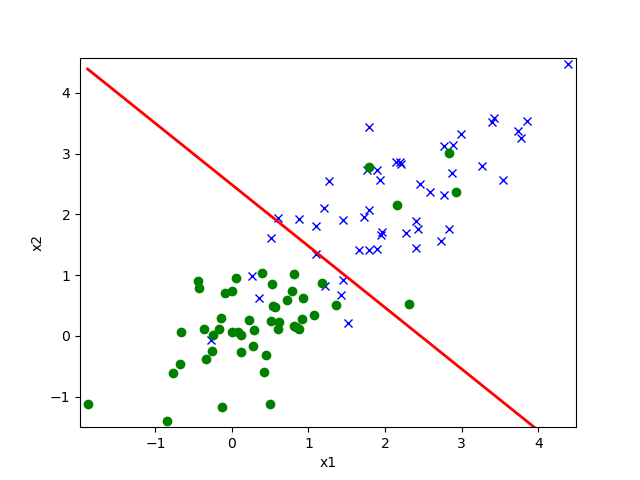
\includegraphics[width=0.65\linewidth]{linearclass/src/p01e_pred_2.png}
    \caption{Separating hyperplane for GDA on Dataset 1 (Note: This is for reference only.  You are not required to submit a plot.)}
\end{figure}

        \ifnum\solutions=1 {
            \input{linearclass/05-solve-gda-sol}
        } \fi

	\item \subquestionpointswritten{1}
For Dataset 1, compare the validation set plots obtained in part (b) and part (e)
from logistic regression and GDA respectively, and briefly comment on your observation in a couple of lines.\\[50pt]

\begin{figure}[H]
    \centering
    \begin{subfigure}{.5\textwidth}
      \centering
      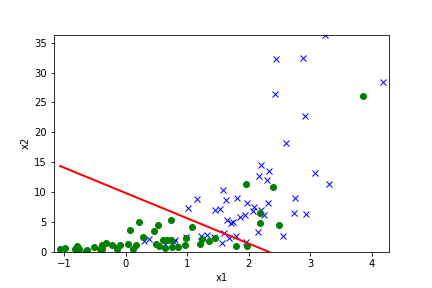
\includegraphics[width=0.95\linewidth]{./linearclass/src/lr_image1.png}
      \caption{Logistic Regression}
    \end{subfigure}%
    \begin{subfigure}{.5\textwidth}
      \centering
      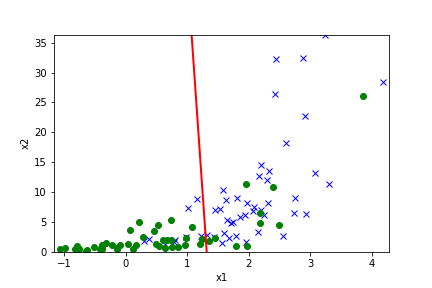
\includegraphics[width=0.95\linewidth]{./linearclass/src/gda_image1.png}
      \caption{GDA}
    \end{subfigure}
    \caption{Dataset 1 Comparison}%
\end{figure}

\hl{Logistic regression did a better job at labeling dataset 1. GDA performed less well because we made the assumption that the covariance matrix $\Sigma$ was identical for both 0 and 1 labels. From the distribution of the data, we can see that it is not Gaussian distribution and 0 and 1 data points do not have identical $\Sigma$.}

        \ifnum\solutions=1 {
            \input{linearclass/06-plot-ds1-sol}
        } \fi

	\item \subquestionpointscodingandwritten{4}
Repeat the steps in part (b) and part (e) for Dataset 2. Create similar plots on
the \textbf{validation set} of Dataset 2 and include those plots in your writeup.

On which dataset does GDA seem to perform worse than logistic regression? Why might this be the case?\\[50pt]

\begin{figure}[H]
    \centering
    \begin{subfigure}{.5\textwidth}
      \centering
      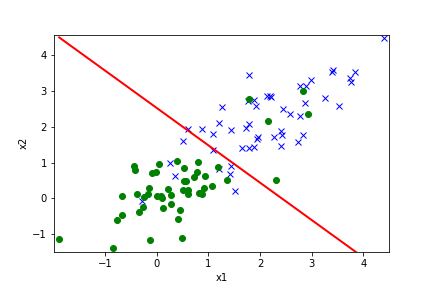
\includegraphics[width=0.95\linewidth]{./linearclass/src/lr_image2.png}
      \caption{Logistic Regression}
    \end{subfigure}%
    \begin{subfigure}{.5\textwidth}
      \centering
      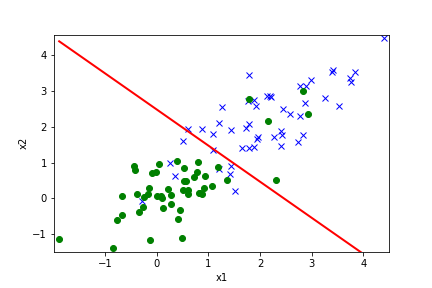
\includegraphics[width=0.95\linewidth]{./linearclass/src/gda_image2.png}
      \caption{GDA}
    \end{subfigure}
    \caption{Dataset 2 Comparison}%
\end{figure}

\hl{GDA performed worse than logistic regression for dataset 1. This is the case because in dataset 1, the data is not Gaussian distributed. GDA performed less well because we made the assumption that the covariance matrix $\Sigma$ was identical for both 0 and 1 labels. From the distribution of the data, we can see that it is not Gaussian distribution and 0 and 1 data points do not have identical $\Sigma$.}

        \ifnum\solutions=1{
            \input{linearclass/07-plot-ds2-sol}
        }\fi

	\item \subquestionpointswritten{1} For the dataset where GDA performed worse in parts (f) and (g), can you find a transformation of the $x^{(i)}$'s such that GDA performs significantly better? What might this transformation be?\\[50pt]

\hl{In dataset 1, x2 seems to have an exponential characteristic. We can apply a transformation to $x^{(i)}$'s such that GDA performs significantly better. The transformation is to apply $\log()$ to x2 in dataset 1.}
        \ifnum\solutions=1{
            \input{linearclass/08-transform-sol}
        }\fi

\end{enumerate}
